\section{Overview}

Markov Decision Process
MDP:
\begin{itemize}
\item State: $S$.
\item Action: $A$.
\item Transition: $P: S \times A \times S \rightarrow \mathcal{R}$.
\item Reward: $R: S \times A \times S \rightarrow \mathcal{R}$.
\end{itemize}

\begin{sidewaystable}
\centering
\begin{tabular}{| l | l | l | l | l |}
  \hline
  Approaches & State & Action & Reward & Value/Q \\
  \hline
  MDP with Option & / & Aggregated actions & / & /\\
  \hline
  Factored MDP & Decomposed states & / & / & Decomposed or not\\
  \hline
  HAM & / & / & / & / \\
  \hline
  Modular RL & / & / & / & / \\
  \hline
\end{tabular}
\label{tbl:overview}
\caption{Overview of decomposition or aggregation of the components of MDP.}
\end{sidewaystable}

\section{Forward Model}

Abstraction on MDP
\begin{itemize}
  \item Aggregate states: feature extraction. 
  \item Aggregate actions: {\bf option}. 
  \item Decompose transition: factored MDP. 
  \item Decompose value (abstract MDP): {\bf HAM, hierarchical RL, modular RL}.
\end{itemize}



MDP with Option
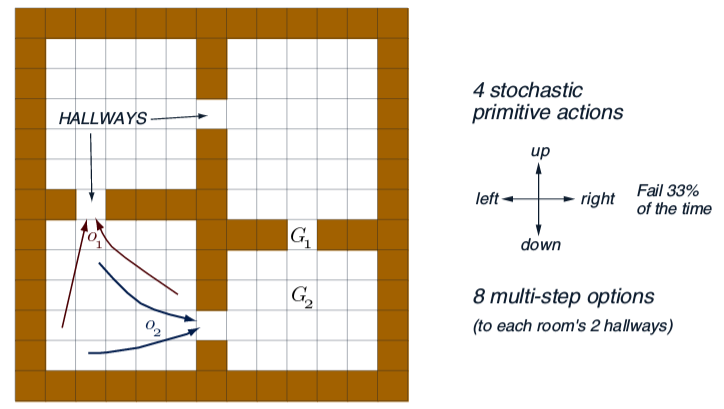
\includegraphics[width=0.8\columnwidth]{option.png}
\begin{itemize}
  \item Option: (start state, policy, termination condition).
\end{itemize}



\begin{itemize}
  \item State: $S$.
  \item Action: $A, {\color{red}O}$.
  \item Transition: $P: S \times {\color{red}\{A, O\}} \times S \rightarrow \mathcal{R}$.
  \item Reward: $R: S \times {\color{red}\{A, O\}} \times S \rightarrow \mathcal{R}$.
\end{itemize}



Hierarchies of Abstract Machines (HAM)
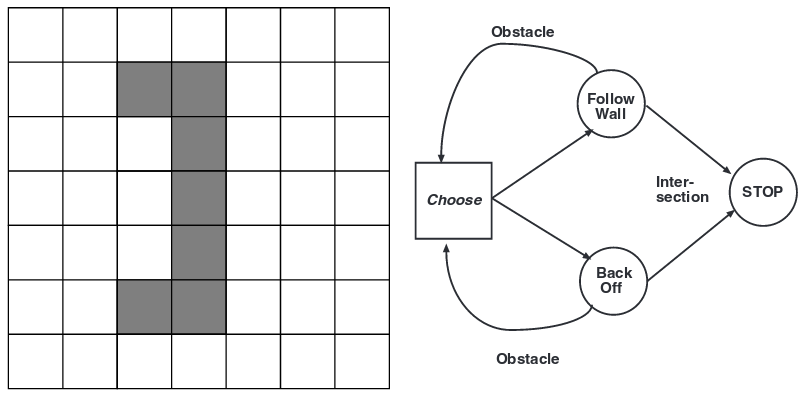
\includegraphics[width=0.8\columnwidth]{ham.png}
\begin{itemize}
  \item State machine of MDPs.
\end{itemize}



Hierarchical RL
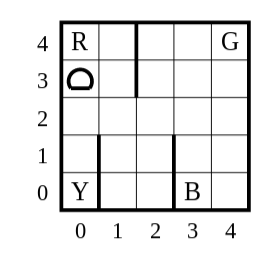
\includegraphics[width=0.4\columnwidth]{taxi.png}

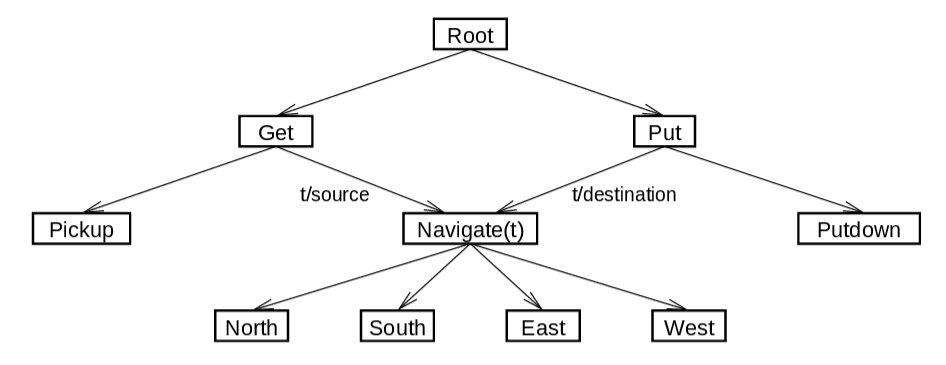
\includegraphics[width=0.8\columnwidth]{maxq.png}



Hierarchical RL
MDP:
\begin{itemize}
  \item State: {\color{red}$\mathcal{S}$}.
  \item Action: {\color{red}$\mathcal{A}$}.
  \item Transition: {\color{red}$\mathcal{T}$}.
  \item Reward: {\color{red}$\mathcal{R}$}.
\end{itemize}



Modular RL
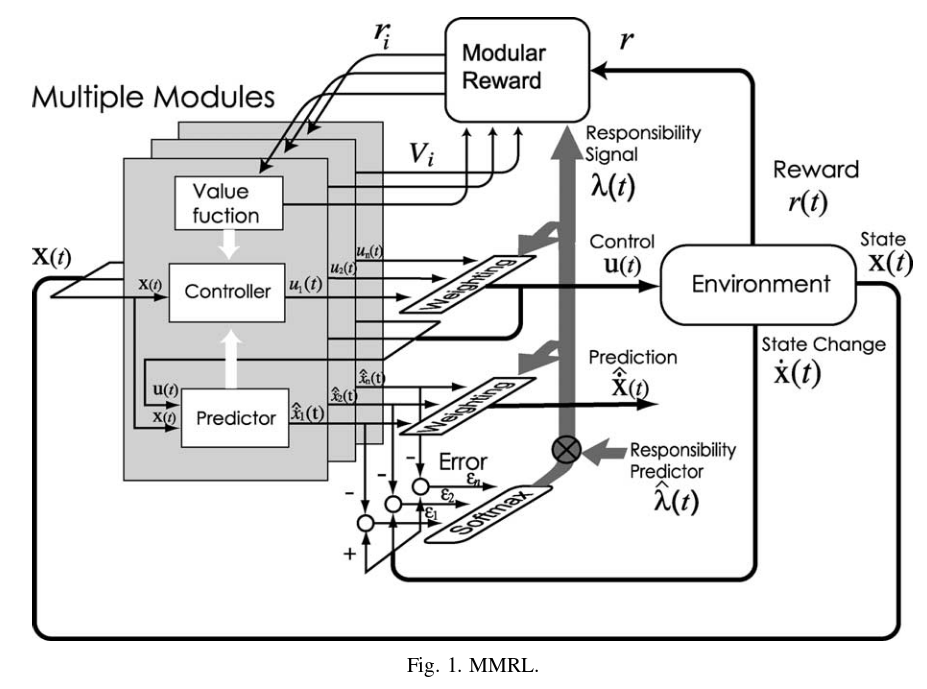
\includegraphics[width=0.8\columnwidth]{mrl.png}



MDP:
\begin{itemize}
  \item State: {\color{red}$S_1 \times S_2 \cdots \times S_M $}.
  \item Action: $A$.
  \item Transition: {\color{red}$P_1 \times P_2 \cdots \times P_M $}.
  \item Reward: {\color{red}$R_1 \times R_2 \cdots \times R_M $}.
\end{itemize}




\section{Ideas in Recent Work}

Not fix a model.

Learn the components,

Dynamic.
